\documentclass[convert={size=640}]{standalone}
\usepackage{tikz}
\usetikzlibrary{arrows}
\usetikzlibrary{arrows.meta}
\usetikzlibrary{shadows}
\usetikzlibrary{positioning}
\usetikzlibrary{calc}
\usetikzlibrary{backgrounds}

\begin{document}

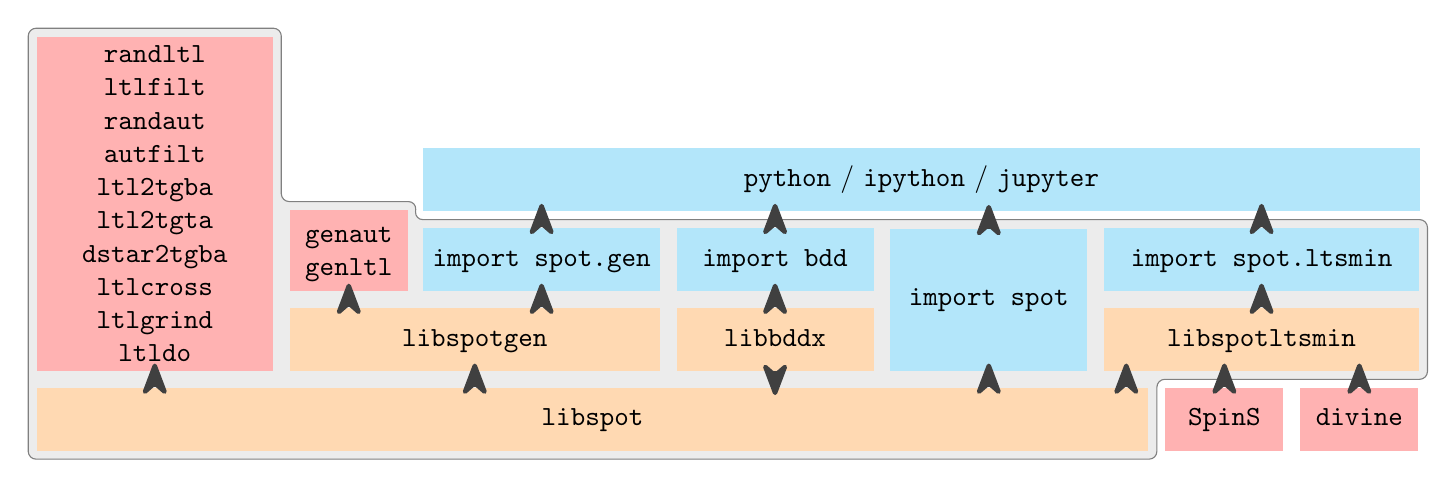
\begin{tikzpicture}
  \tikzset{node distance=2mm,
           basicbox/.style={minimum width=#1,minimum height=8mm},
           double height/.style={minimum height=18mm},
           cppbox/.style={basicbox=#1,fill=orange!30},
           pybox/.style={basicbox=#1,fill=cyan!30},
           shbox/.style={basicbox=#1,fill=red!30},
           usedby/.style={->,ultra thick,>={Stealth[length=5mm,round]},gray!50!black}}
  \node[cppbox=14.12cm] (libspot) {\texttt{libspot\strut}};
  \node[shbox=3cm,above right=2mm and 0mm of libspot.north west,align=center] (shcmd) {
    \texttt{randltl}\\
    \texttt{ltlfilt}\\
    \texttt{randaut}\\
    \texttt{autfilt}\\
    \texttt{ltl2tgba}\\
    \texttt{ltl2tgta}\\
    \texttt{dstar2tgba}\\
    \texttt{ltlcross}\\
    \texttt{ltlgrind}\\
    \texttt{ltldo}
  };
  \node[cppbox=4.7cm,above right=0mm and 2mm of shcmd.south east] (libgen) {\texttt{libspotgen\strut}};
  \node[cppbox=2.5cm,above right=0mm and 2mm of libgen.south east] (buddy) {\texttt{libbddx\strut}};
  \node[pybox=2.5cm,above right=0mm and 2mm of buddy.south east,double height] (pyspot) {\texttt{import spot}};
  \node[cppbox=4cm,above right=0mm and 2mm of pyspot.south east] (libltsmin) {\texttt{libspotltsmin\strut}};

  \node[shbox=1.5cm,above right=2mm and 0mm of libgen.north west,align=center] (genaut) {
    \texttt{genaut\strut}\\
    \texttt{genltl}
  };

  \node[pybox=3cm,above left=2mm and 0mm of libgen.north east] (pygen) {\texttt{import spot.gen\strut}};
  \node[pybox=2.5cm,above=of buddy] (pybuddy) {\texttt{import bdd\strut}};

  \node[pybox=4cm,above=2mm] (pyltsmin) at (libltsmin.north) {\texttt{import spot.ltsmin\strut}};
  \node[shbox=1.5cm,right=of libspot] (spins) {\texttt{SpinS\strut}};
  \node[shbox=1.5cm,right=of spins] (divine) {\texttt{divine\strut}};

  \node[pybox=12.65cm,above right=2mm and 0mm of pygen.north west] (ipython) {\texttt{python} / \texttt{ipython} / \texttt{jupyter}};

  \draw[usedby] (buddy.north) -- ++(0,3mm);
  \draw[usedby] (buddy.south) -- ++(0,-3mm);
  \draw[usedby] (pybuddy.north) -- ++(0,3mm);
  \draw[usedby] (spins.north) -- ++(0,3mm);
  \draw[usedby] (divine.north) -- ++(0,3mm);
  \draw[usedby] (libgen.south |- libspot.north) -- ++(0,3mm);
  \draw[usedby] (genaut.south |- libgen.north) -- ++(0,3mm);
  \draw[usedby] (pygen.south |- libgen.north) -- ++(0,3mm);
  \draw[usedby] (pygen.north) -- ++(0,3mm);
  \draw[usedby] (pyspot.south) ++(0,-2mm) -- ++(0,3mm);
  \draw[usedby] (pyltsmin.south) ++(0,-2mm) -- ++(0,3mm);
  \draw[usedby] (shcmd.south) ++(0,-2mm) -- ++(0,3mm);
  \draw[usedby] (pyspot.north) -- ++(0,3mm);
  \draw[usedby] (pyltsmin.north) -- ++(0,3mm);
  \coordinate (x) at ($(libltsmin.south west)!.5!(libspot.north east)$);
  \draw[usedby] (libspot.north -| x) -- ++(0,3mm);

\begin{pgfonlayer}{background}
\path[fill=gray!15,draw=gray,rounded corners=1mm]
($(shcmd.north west)+(-1mm,1mm)$) --
($(shcmd.north east)+(1mm,1mm)$) --
($(genaut.north west)+(-1mm,1mm)$) --
($(genaut.north east)+(1mm,1mm)$) --
($(pygen.north west)+(-1mm,1mm)$) --
($(pyltsmin.north east)+(1mm,1mm)$) --
($(libltsmin.south east)+(1mm,-1mm)$) --
($(libspot.north east)+(1mm,1mm)$) --
($(libspot.south east)+(1mm,-1mm)$) --
($(libspot.south west)+(-1mm,-1mm)$) -- cycle;
\end{pgfonlayer}
\end{tikzpicture}
\end{document}
%%% Local Variables:
%%% mode: latex
%%% TeX-master: t
%%% End:
